\documentclass[10pt]{beamer}

%% Chinese support
%% \usepackage[adobefonts,nocap]{ctex}

%% Fonts
\usepackage{multicol}
\usepackage{mathabx}
\usepackage[scaled]{helvet}
\usepackage{lmodern}
\usepackage{eulervm}
\usefonttheme[onlymath]{serif}
\usefonttheme{professionalfonts}
\usefonttheme{structurebold}
\usepackage{bm}
\usepackage{verbatim}

%% Color & Theme
\definecolor{SUblue}{RGB}{0,0,180}
\usecolortheme[RGB={0,0,180}]{structure}
\usetheme{Boadilla}
\setbeamertemplate{navigation symbols}{}
\setbeamertemplate{itemize items}[circle]
\setbeamertemplate{enumerate items}[circle]
\setbeamerfont{title}{size=\large}
\setbeamerfont{frametitle}{size=\large}
\setbeamerfont{framesubtitle}{size=\large,shape =$\color{violet}{\looparrowdownright}~$}
\setbeamercolor{title}{fg=white, bg= SUblue!75!green}
\setbeamercolor{framesubtitle}{fg=violet}
% \setlength{\leftmargini}{5pt}


\title[Statistical Computing]{{\textbf{Sampling with Markov chain Monte Carlo}}}

\author[Feng Li]{
\includegraphics[height=2cm]{cufelogo}\\
  \vspace{0.5cm}\textbf{Feng Li\\\texttt{feng.li@cufe.edu.cn}}}

\institute[SAM.CUFE.EDU.CN]{\footnotesize{\textbf{School of
      Statistics and Mathematics\\ Central University of Finance and
      Economics}}}

\date{}
%%%%%%%%%%%%%%%%%%%%%%%%%%%%%%%%%%%%%%%%%%%%%%%%%%%%%%%%%%%%%%%%%%%%%%
\begin{document}

%% Title page
\begin{frame}[plain]
  \titlepage
  \tiny{Revised on \today}
\end{frame}


%% Outline page
\section*{Today we are going to learn...}
\begin{frame}
  \frametitle{Today we are going to learn...}
  \tableofcontents
\end{frame}

\begin{frame}{Markov Chains}
\begin{itemize}
\item The goal of today's lecture is to learn about the {\bf Metropolis Hastings algorithm}

\item The Metropolis Hastings algorithm allows us to simulate from any distribution as long as we have the kernel of the density of the distribution.

\item To understand the Metropolis Hastings algorithm,  we must learn a little bit about {\bf Markov chains}
\end{itemize}
\end{frame}

\begin{frame}{Basic Probability Rules}

  \begin{itemize}
  \item
\textbf{Law of conditional probability}
\begin{equation}
\mbox{Pr}(A=a,B=b)=\mbox{Pr}(A=a|B=b)\mbox{Pr}(B=b)
\end{equation}

\item More general conditional probability
\begin{align}
\mbox{Pr}(A=a,B=b|C=c)=\mbox{Pr}&(A=a|B=b,C=c)\times\nonumber\\
&\mbox{Pr}(B=b|C=c)
\end{align}
  \end{itemize}

\end{frame}
\begin{frame}{Basic Probability Rules}
  \begin{itemize}
  \item
  \textbf{Marginalizing} (for a discrete variable)
\begin{equation}
\mbox{Pr}(A=a)=\sum_{b}\mbox{Pr}(A=a,B=b)
\end{equation}

\item More general
\begin{equation}
\mbox{Pr}(A=a|C=c)=\sum_{b}\mbox{Pr}(A=a,B=b|C=c)
\end{equation}
  \end{itemize}

\end{frame}
\begin{frame}{Independence}
  \begin{itemize}
  \item
Two variables are {\bf independent} if
\begin{equation}
\mbox{Pr}(A=a,B=b)=\mbox{Pr}(A=a)\mbox{Pr}(B=b)\quad\forall a,b
\end{equation}

\item Dividing both sides by \mbox{Pr}(B=b) gives
\begin{equation}
\mbox{Pr}(A=a|B=b)=\mbox{Pr}(A=a)\quad\forall a,b
\end{equation}
  \end{itemize}
\end{frame}
\begin{frame}{Conditional Independence}
  \begin{itemize}
  \item
Two variables A and B are {\bf Conditionally Independent} if
\begin{align}
\mbox{Pr}(A=a,B=b|C=c)=\mbox{Pr}&(A=a|C=c)\times\nonumber\\&\mbox{Pr}(B=b|C=c)\quad\forall a,b,c
\end{align}

\item Dividing both sides by $\mbox{Pr}(B=b|C=c)$ gives
\begin{equation}
\mbox{Pr}(A=a|B=b,C=c)=\mbox{Pr}(A=a|C=c)\quad\forall a,b,c
\end{equation}
  \end{itemize}
\end{frame}
\section{Markov Chains}
\begin{frame}{A simple game}
\begin{itemize}
\item Player A and Player B play a game.  The probability that Player A wins each game is 0.6 and the probability that Player B wins each game is 0.4.
\item They play the game $N$ times.
\item Each game is {\bf independent}.
\item Let

\begin{itemize}
\item $X_i=0$ if Player A wins game $i$
\item $X_i=1$ if Player B wins game $i$
\end{itemize}

\item Also assume there is an initial Game called Game 0 ($X_0$)
\end{itemize}
\end{frame}
\begin{frame}{Some simple questions}
\begin{itemize}
\item What is the probability that Player A wins  Game 1 ($(X_1=0)$) if

\begin{itemize}
\item If $X_0=0$ (Player A wins Game 0)

\item If $X_0=1$ (Player B wins Game 0)
\end{itemize}

\item What is the probability that Player A wins Game 2 ($(X_2=0)$) if

\begin{itemize}
\item If $X_0=0$ (Player A wins Game 0)

\item If $X_0=1$ (Player B wins Game 0)
\end{itemize}

\item Since each game is independent all answers are 0.6.
\end{itemize}
\end{frame}
\begin{frame}{A different game: A Markov chain}
\begin{itemize}
\item Now assume that both players have a better chance of winning Game $i+1$ if they already won Game $i$.

\begin{align}
\mbox{Pr}(X_{i+1}=0|X_{i}=0)&=0.8\\
\mbox{Pr}(X_{i+1}=1|X_{i}=1)&=0.7
\end{align}

\item Assume nothing other than game $i$ has a direct effect on Game $i+1$.

\item This is called the {\bf Markov Property}. Mathematically

\begin{equation}
\mbox{Pr}(X_{i+1}|X_{i},X_{i-1},\ldots,X_{1},X_{0})=\mbox{Pr}(X_{i+1}|X_{i})
\end{equation}
\end{itemize}
\end{frame}
\begin{frame}{Markov Property}
\begin{itemize}
\item Another way to define the Markov property is to notice that $X_{i+1}$ and $X_{i-1},\ldots,X_{0}$ are {\bf independent} conditional on $X_{i}$

\item This may be a model for the stock market, all the valuable information about tomorrow's stock price is contained in today's price.

\item This is related to the {\bf Efficient Market Hypothesis}, a popular theory in finance.

\item Now back to the simple game.
\end{itemize}
\end{frame}
\begin{frame}{Simulating from a Markov chain}
\begin{itemize}
\item Now let's simulate a sequence $X_1,X_2,\ldots,X_{100}$ from the Markov chain.

\item Initialize at $x_0=0$.  Then inside a loop

\item Code the following using {\em if}.
\begin{itemize}
\item if $X_i=0$ then $X_{i+1}=\left\{
\begin{array}{c}
0\quad\mbox{with probability 0.8 }\\
1\quad\mbox{with probability 0.2 }\\
\end{array}
\right.$
\item if $X_i=1$ then $X_{i+1}=\left\{
\begin{array}{c}
0\quad\mbox{with probability 0.3 }\\
1\quad\mbox{with probability 0.7 }\\
\end{array}
\right.$
\end{itemize}

\item Try it
\end{itemize}
\end{frame}
\begin{frame}{Markov chain}
\begin{center}
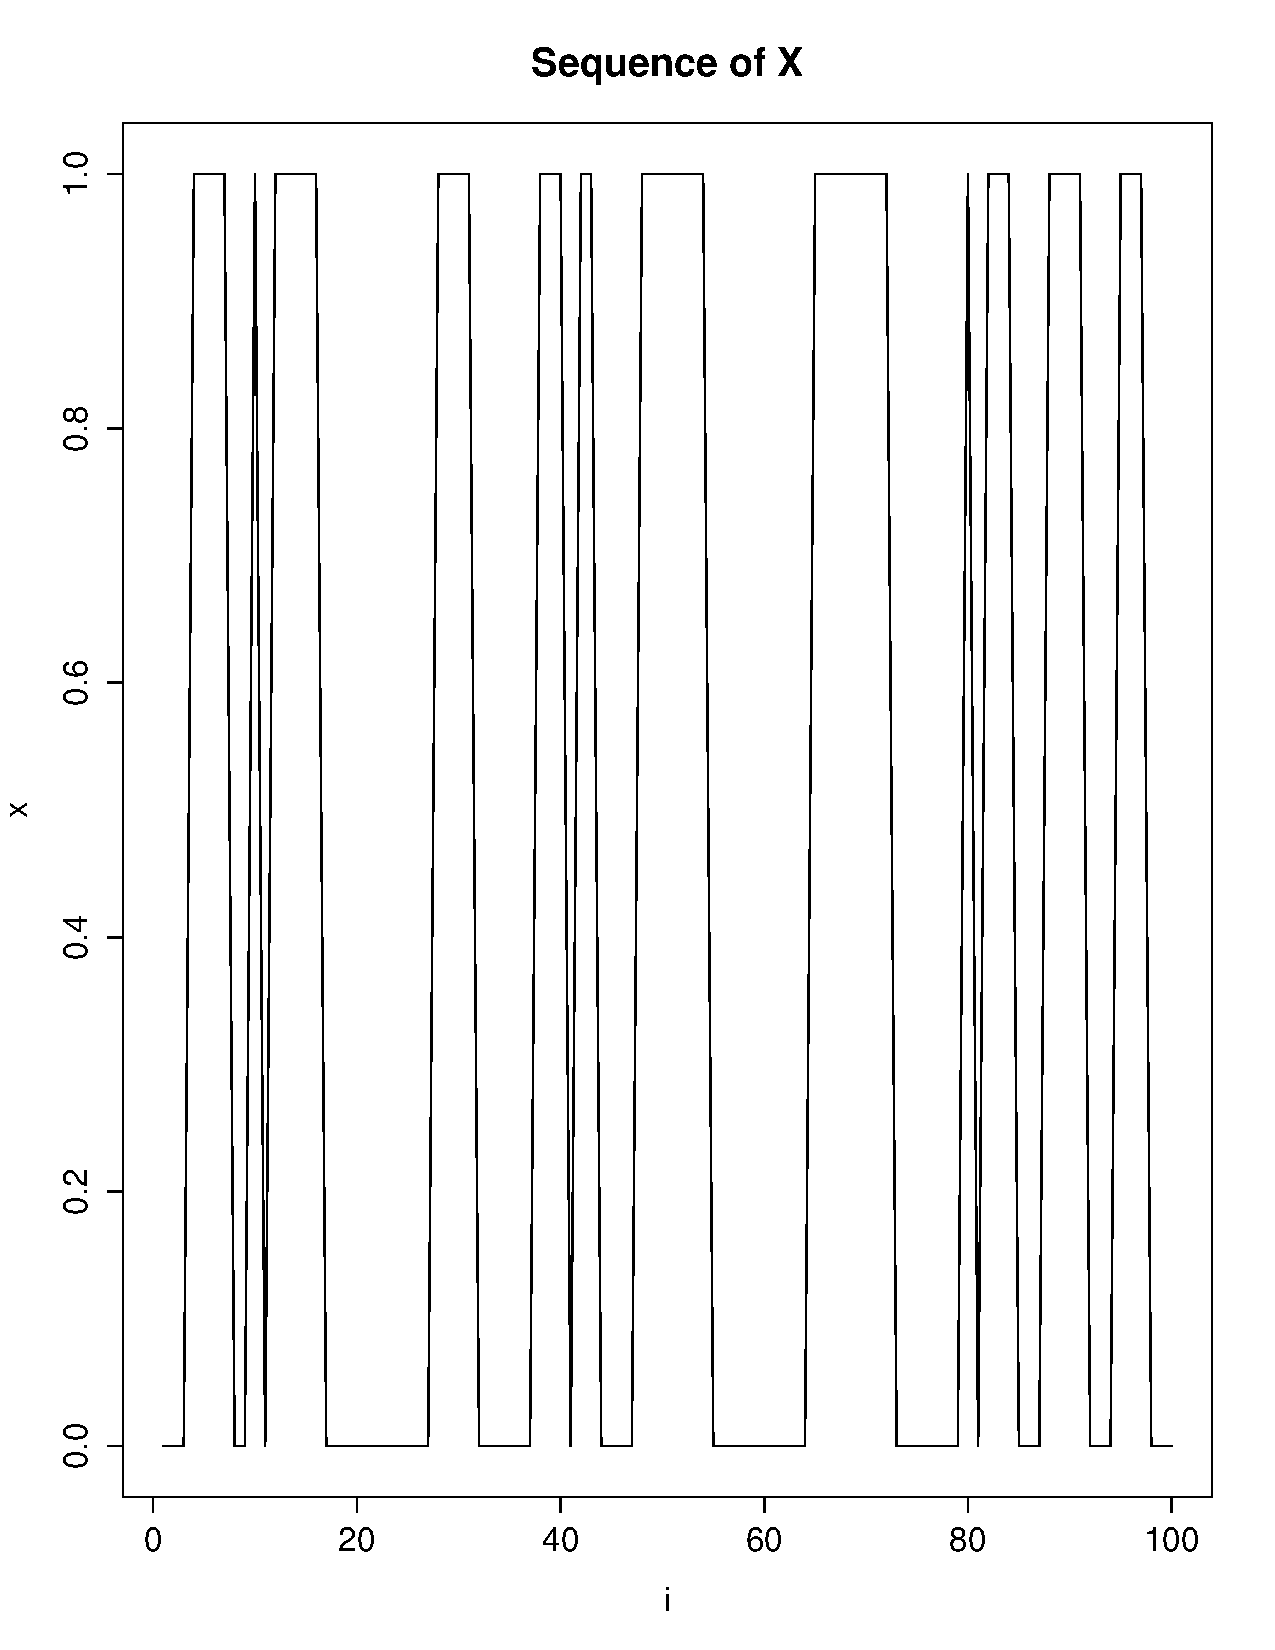
\includegraphics[height=7cm]{./Pics/seqx.pdf}
\end{center}
\end{frame}
\begin{frame}{Simple questions again}
\begin{itemize}
\item What is the probability that Player A wins the first game (i.e $(X_1=0)$) if

\begin{itemize}
\item If $X_0=0$ (Player A wins initial game)

\item If $X_0=1$ (Player B wins initial game)
\end{itemize}

\item The answers are 0.8 and 0.3.

\item What is the probability that Player A wins the second game $(X_2=0)$ if

\begin{itemize}
\item If $X_0=0$ (Player A wins initial game)

\item If $X_0=1$ (Player B wins initial game)
\end{itemize}
\end{itemize}
\end{frame}
\begin{frame}{Solution}
\begin{itemize}
\item Let $X_0=0$.  Then $\mbox{Pr}(X_2=0|X_0=0)$

\begin{align*}
&=\sum_{x_1=0,1}\mbox{Pr}(X_2=0,X_1=x_1|X_0=0)\\
&=\sum_{x_1=0,1}\mbox{Pr}(X_2=0|X_1=x_1,X_0=0)
%\nonumber\\
%&\quad\quad\quad\quad
\mbox{Pr}(X_1=x_1|X_0=0)\\
&=\sum_{x_1=0,1}\mbox{Pr}(X_2=0|X_1=x_1)\mbox{Pr}(X_1=x_1|X_0=0)\\
&=0.8\times 0.8+0.3\times 0.2\\
&=0.7
\end{align*}

\item What if $X_0=1$?
\end{itemize}
\end{frame}
\begin{frame}{Recursion}
\begin{itemize}
\item Notice that the distribution of $X_i$ depends on $X_0$

\item The sequence is no longer independent.

\item How could you compute $\mbox{Pr}(X_n=0|X_0=0)$ when $n=3$, when $n=5$, when $n=100$?

\item This is hard, but the Markov Property does make things simpler

\item We can use a recursion to compute the probability that Player A wins any game.
\end{itemize}
\end{frame}
\begin{frame}{Recursion}
Note that $\mbox{Pr}(X_i=0|X_0=0)$

\begin{align*}
=&\sum_{x_{i-1}}\mbox{Pr}(X_i=0,X_{i-1}=x_{i-1}|X_0=0)\\
=&\sum_{x_{i-1}}\mbox{Pr}(X_i=0|X_{i-1}=x_{i-1},X_0=0)\mbox{Pr}(X_{i-1}=x_{i-1}|X_0=0)\\
=&\sum_{x_{i-1}}\mbox{Pr}(X_i=0|X_{i-1}=x_{i-1})\mbox{Pr}(X_{i-1}=x_{i-1}|X_0=0)\\
\end{align*}

We already applied this formula when $i=2$.  We can continue for $i=3,4,5,\ldots,n$
\end{frame}
\begin{frame}{Recursion}
\begin{equation*}
\mbox{Pr}(X_i=0|X_0=0)=\sum_{x_{i-1}}\mbox{Pr}(X_i=0|X_{i-1}=x_{i-1})\mbox{Pr}(X_{i-1}=x_{i-1}|X_0=0)
\end{equation*}

\begin{itemize}
\item Start with $\mbox{Pr}(X_1=0|X_0=0)$

\item Get $\mbox{Pr}(X_1=1|X_0=0)$

\item Use these in formula with $i=2$

\item Get $\mbox{Pr}(X_2=0|X_0=0)$

\item Get $\mbox{Pr}(X_2=1|X_0=0)$

\item Use these in formula with $i=3$

\item Get $\mbox{Pr}(X_3=0|X_0=0)$

\item $\vdots\quad\quad\vdots\quad\quad\vdots\quad\quad\vdots$
\end{itemize}
\end{frame}
\begin{frame}{Matrix Form}
It is much easier to do this calculation in matrix form (especially when $X$ is not binary).  Let $P$ be the transition matrix

\begin{table}
\begin{center}
\begin{tabular}{c|cc}
& $X_{i}=0$ & $X_{i}=1$\\
\hline
$X_{i-1}=0$ & $\mbox{Pr}(X_{i}=0|X_{i-1}=0)$ & $\mbox{Pr}(X_{i}=1|X_{i-1}=0)$\\
$X_{i-1}=1$ & $\mbox{Pr}(X_{i}=0|X_{i-1}=1)$ & $\mbox{Pr}(X_{i}=1|X_{i-1}=1)$\\
\end{tabular}
\end{center}
\end{table}
\end{frame}
\begin{frame}{Matrix Form}
In our example:

\begin{table}
\begin{center}
\begin{tabular}{c|cc}
& $X_{i}=0$ & $X_{i}=1$\\
\hline
$X_{i-1}=0$ & $0.8$ & $0.2$\\
$X_{i-1}=1$ & $0.3$ & $0.7$\\
\end{tabular}
\end{center}
\end{table}

\begin{equation}
P=\left(
\begin{array}{cc}
0.8 & 0.2\\0.3 & 0.7\\
\end{array}
\right)
\end{equation}
\end{frame}
\begin{frame}{Matrix Form}
Let $\pi_i$ be a $1\times 2$ row vector which denotes the probabilities of each player winning Game $i$ conditional on the initial Game

\begin{equation}
\pi_i=\left(\mbox{Pr}(X_i=0|X_0),
\,\mbox{Pr}(X_i=1|X_0)\right)
\end{equation}

In our example if $X_0=0$

\begin{equation}
\pi_1=\left(0.8,
\, 0.2\right)
\end{equation}

In our example if $X_0=1$

\begin{equation}
\pi_1=\left(0.3,\, 0.7\right)
\end{equation}
\end{frame}
\begin{frame}{Recursion in Matrix form}
\begin{itemize}
\item The recursion formula is

\begin{equation}
\pi_{i}=\pi_{i-1}P
\end{equation}

Therefore

\begin{equation}
\pi_{n}=\pi_{1}P\times P\times\ldots\times P
\end{equation}

\item Now code this up in R.

\item What is $\mbox{Pr}(X_n=0|X_0=0)$ when
\begin{itemize}
\item $n=3$
\item $n=5$
\item $n=100$?
\end{itemize}

\item Do the same when $X_0=1$
\end{itemize}
\end{frame}
\begin{frame}{Convergence?}
\begin{itemize}
\item For $n=3$ and $n=5$, the starting point made a big difference.

\item For $n=100$ it did not make a big difference.

\item Could this Markov chain be converging to something?

\item Now write code to keep the values of $\pi_i$ for $i=1,2,\ldots,100$.

\item Then plot the values of $\pi_{i1}$ against $i$
\end{itemize}
\end{frame}
\begin{frame}{Convergence}
\begin{center}
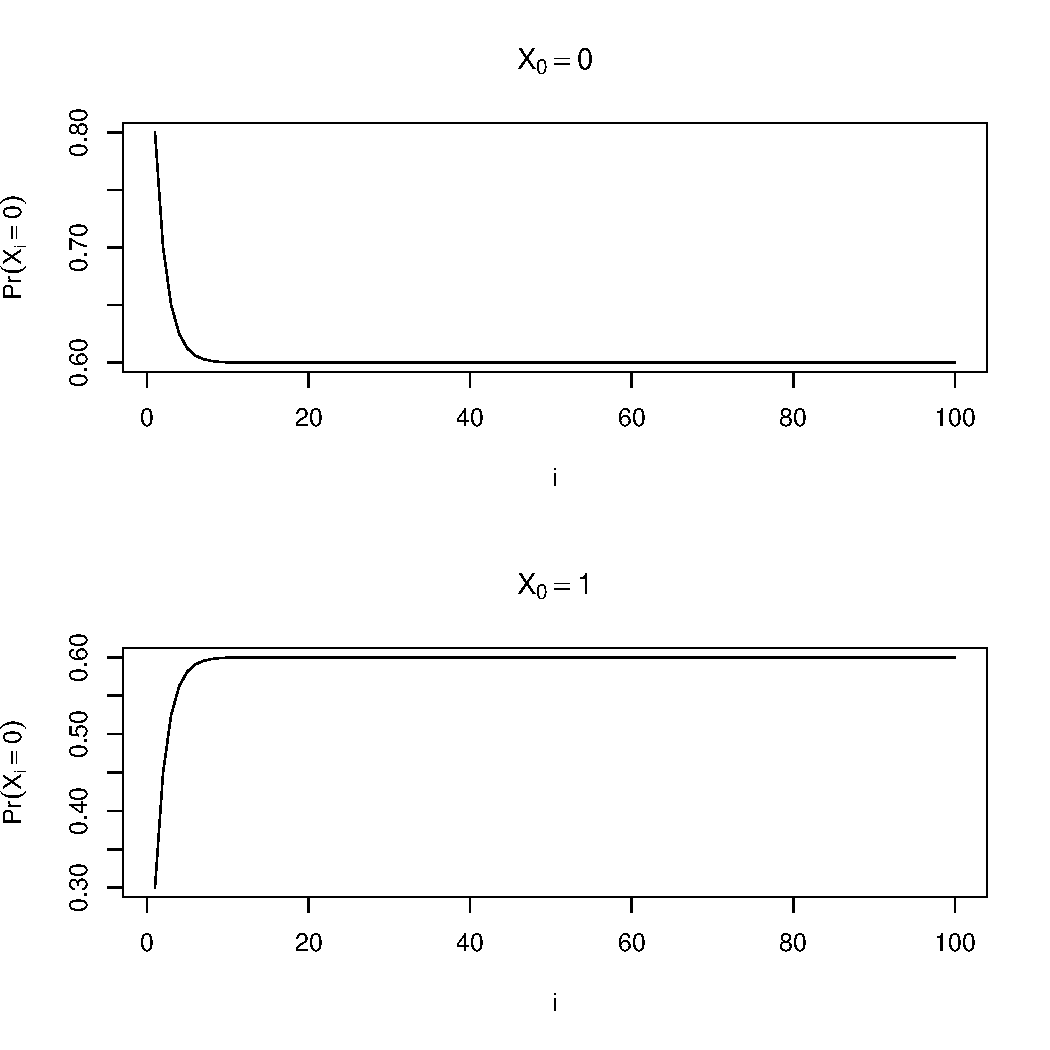
\includegraphics[height=7cm]{Pics/MarkovConv.pdf}
\end{center}
\end{frame}
\begin{frame}{More Questions}
\begin{itemize}
\item What is $Pr(X_{100}=0|X_0=0)$?

\item What is $Pr(X_{100}=0|X_0=1)$?

\item What is $Pr(X_{1000}=0|X_0=0)$?

\item What is $Pr(X_{1000}=0|X_0=1)$?

\item The answer to all of these is 0.6.

\item The $X$ do not converge.  They keep changing from 0 to 1.  The Markov chain however converges to a {\bf stationary distribution}.
\end{itemize}
\end{frame}
\begin{frame}{Simulation with  a Markov chain}
\begin{itemize}
\item Go back to your code for generating a Markov chain and generate a chain with $n=110000$

\item Exclude the first 10000 values of $X_i$ and keep the remaining 100000 values.

\item How many $X_i=0$? How many $X_i=1$

\item We have discovered a new way to simulate from a distribution with $\mbox{Pr}(X_i=0)=0.6$
and $\mbox{Pr}(X_i=1)=0.4$
\end{itemize}
\end{frame}
\begin{frame}{Markov Chains}
\begin{itemize}
\item Sometimes two different Markov chains converge to the same stationary distribution.  See what happens when

\begin{equation}
P=\left(
\begin{array}{cc}
0.9 & 0.1\\0.15 & 0.85\\
\end{array}
\right)
\end{equation}

\item Sometimes Markov chains do not converge to a stationary distribution at all.

\item Some Markov chains can get stuck in an {\bf absorbing state}.  For example what would the simple example look like if $\mbox{Pr}(X_{i+1}=0|X_{i}=0)=1$?

\item Markov chains can be defined on continuous support as well, $X_i$ can be continuous.
\end{itemize}
\end{frame}
\begin{frame}{Some important points}
\begin{itemize}
\item This is a very complicated way to generate from a simple distribution.

\item For the binary example the direct method would be better.

\item However for other examples, either the direct method or accept/reject algorithm do not work.

\item In these cases we can construct a Markov chain that has a stationary distribution that is our {\bf target distribution}.

\item All we need is the kernel of the density function, and an algorithm called the {\bf Metropolis Algorithm}
\end{itemize}
\end{frame}
\begin{frame}{Normalizing Constant and Kernel}
What are the
\alt<1>{ normalizing constant}{{\color{blue} normalizing constant}}
and
\alt<1>{kernel}{{\color{red} kernel}}
of the Beta density?
\alt<1>{
\begin{equation}
\mbox{Beta}(x;a,b)=\frac{\Gamma(a+b)}{(\Gamma(a)\Gamma(b))}x^{a-1}(1-x)^{b-1}
\end{equation}
}{
\begin{equation}
\mbox{Beta}(x;a,b)={\color{blue}\frac{\Gamma(a+b)}{(\Gamma(a)\Gamma(b))}}{\color{red}x^{a-1}(1-x)^{b-1}}
\end{equation}
}

\end{frame}
\section{Metropolis Algorithm}
\begin{frame}{The Metropolis algorithm}
\begin{itemize}
\item The Metropolis algorithm was developed in a 1953 paper by Metropolis, Rosenbluth, Rosenbluth, Teller and Teller.

\item The aim is to simulate $x\sim p(x)$ where $p(x)$ is called the {\bf target density}.

\item We will need a {\bf proposal density} $q(x^{[old]}\rightarrow x^{[new]})$

\item For example one choice of $q$ is

\begin{equation}
x^{[new]}\sim N(x^{[old]},1)
\end{equation}

\item This is called a {\bf Random Walk proposal}
\end{itemize}
\end{frame}
\begin{frame}{Symmetric proposal}
\begin{itemize}
\item An important property of $q$ in the Metropolis algorithm is symmetry of the proposal

\begin{equation}
q(x^{[old]}\rightarrow x^{[new]})=q(x^{[new]}\rightarrow x^{[old]})
\end{equation}

\item Later we will not need this  assumption

\item Can you confirm this is true for $x^{[new]}\sim N(x^{[old]},1)$?

\item Can you simulate from this random walk (use $x_0=0$ as a starting value)?
\end{itemize}
\end{frame}
\begin{frame}{Proof of symmetry of random walk}
The proposal
\begin{align}
q(x^{[old]}\rightarrow x^{[new]})&=(2\pi)^{-1/2}exp\left\{-\frac{1}{2}\left(x^{[new]}-x^{[old]}\right)^2\right\}\\
&=(2\pi)^{-1/2}exp\left\{-\frac{1}{2}\left[-1\left(x^{[new]}-x^{[old]}\right)\right]^2\right\}\\
&=(2\pi)^{-1/2}exp\left\{-\frac{1}{2}\left(x^{[old]}-x^{[new]}\right)^2\right\}\\
&=q(x^{[new]}\rightarrow x^{[old]})
\end{align}
\end{frame}
\begin{frame}{Accept and reject}
\begin{itemize}
\item By itself the random walk will not converge to anything.

\item To make sure this Markov chain converges to our target, we need to include the following.

\item At step $i+1$ set $x^{[old]}=x^{[i]}$.

\item Generate $x^{[new]}\sim N(x^{[old]},1)$ and compute

\begin{equation}
\alpha=min\left(1,\frac{p(x^{[new]})}{p(x^{[old]})}\right)
\end{equation}

\item Then

\begin{itemize}
\item Set $x^{[i+1]}$ to $x^{[new]}$ with probability $\alpha$ (accept)

\item Set $x^{[i+1]}$ to $x^{[old]}$ with probability $1-\alpha$ (reject)
\end{itemize}
\end{itemize}
\end{frame}
\begin{frame}{Code it up}
\begin{itemize}
\item Use the Metropolis algorithm with a random walk proposal to simulate a sample from the standard t distribution with 5 df.

\item The target density is
\begin{equation}
p(x)=\left[1+\frac{x^2}{5}\right]^{-3}
\end{equation}

\item Simulate a Markov chain with 110000 iterates using the random walk as a proposal.

\item The first 10000 iterates are the {\bf burn-in} and will be left out because the Markov chain may not have converged yet.

\item Use $x_0=0$ as a starting value
\end{itemize}
\end{frame}
\begin{frame}{Some diagnostics - Convergence}
\begin{itemize}
\item There a few diagnostics we can use to investigate the behaviour of the chain

\item One is a trace plot (including burn in), which is simply a line plot of the iterates.

\item Plot this for your Markov chain

\item Another diagnostic is the {\bf Geweke diagnostic} which can be found in the R package {\em coda}.

\item The Geweke diagnostic tests the equality of the means of two different parts of the chain (excluding burn-in). The test statistic has a standard normal distribution.

\item Rejecting this test is evidence that the chain has not converged
\end{itemize}
\end{frame}
\begin{frame}{Trace Plot}
\begin{center}
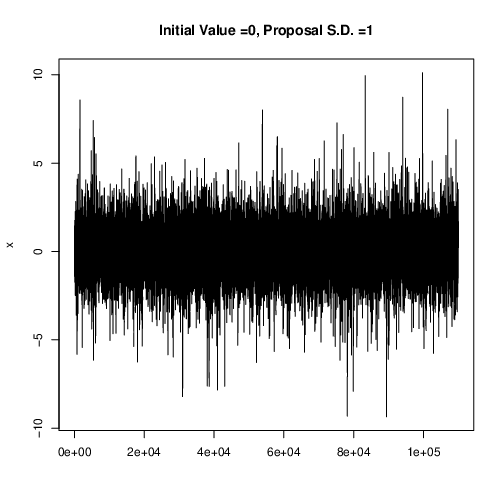
\includegraphics[height=7cm]{./Pics/sp1.png}
\end{center}
\end{frame}
\begin{frame}{The effect of starting value}
\begin{itemize}
\item Now rerun the code with a starting value of $X_0=100$

\item Does the chain still converge?

\item Does it converge quicker or slower?
\end{itemize}
\end{frame}
\begin{frame}{Trace Plot}
\begin{center}
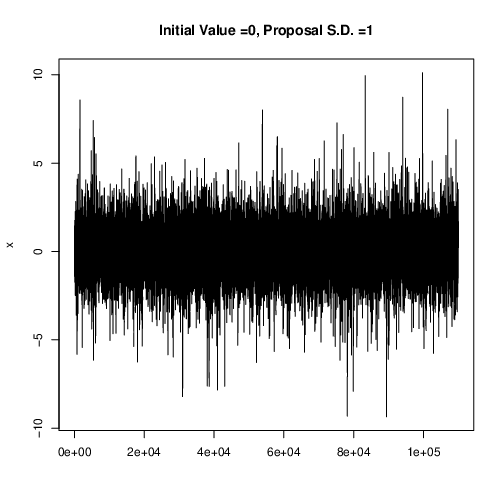
\includegraphics[height=7cm]{./Pics/sp1.png}
\end{center}
\end{frame}
\begin{frame}{Trace Plot}
\begin{center}
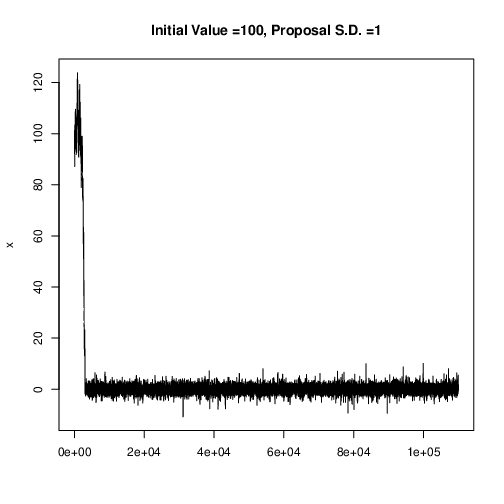
\includegraphics[height=7cm]{./Pics/sp2.png}
\end{center}
\end{frame}
\begin{frame}{The effect of proposal variance}
\begin{itemize}
\item Keep the starting value of $X_0=100$

\item No change the standard deviation of the proposal to 3.

\item Does the chain still converge?

\item Does it converge quicker or slower?
\end{itemize}
\end{frame}
\begin{frame}{Trace Plot}
\begin{center}
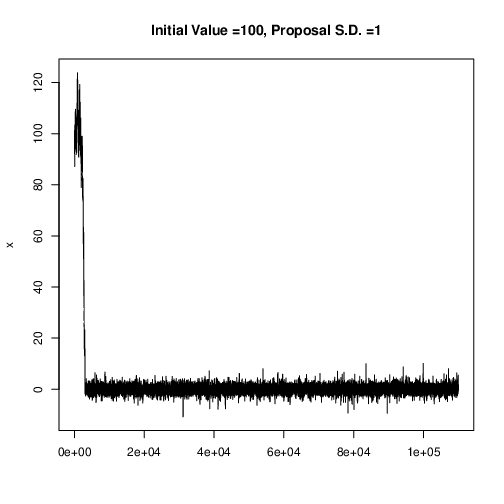
\includegraphics[height=7cm]{./Pics/sp2.png}
\end{center}
\end{frame}
\begin{frame}{Trace Plot}
\begin{center}
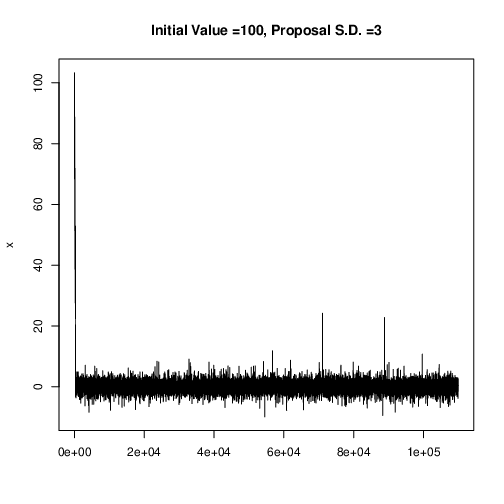
\includegraphics[height=7cm]{./Pics/sp3.png}
\end{center}
\end{frame}
\begin{frame}{Huge proposal variance}
\begin{itemize}
\item Maybe you think the best strategy is to choose a huge standard deviation.

\item Try to use a proposal standard deviation of 100.  Plot a trace plot of the chain.

\item The plot is rejecting many iterates.  This must be inefficient

\item Change your code to compute the percentage of times a new iterate is accepted (excluding burn in).

\item Use $x_0=$ as an initial value.  What is the acceptance rate when the proposal standard deviation is 1?  What is the acceptance rate when the proposal standard deviation is 100?
\end{itemize}
\end{frame}
\begin{frame}{Trace Plot}
\begin{center}
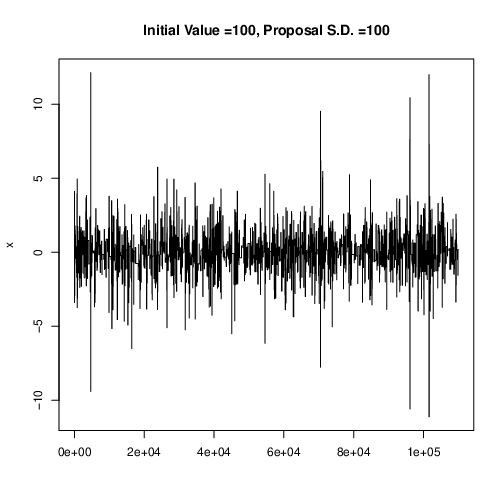
\includegraphics[height=7cm]{./Pics/sp4.png}
\end{center}
\end{frame}
\begin{frame}{Acceptance Rate}
\begin{itemize}
\item If the proposal variance is too high

\begin{itemize}
\item Values will be proposed that are too far into the tails of the stationary distribution

\item The Metropolis algorithm will mostly reject these values.

\item The sample will still come from the  correct target distribution but this is a very inefficient way to sample.
\end{itemize}

\item What happens if a very small proposal variance is used.

\item Try a proposal variance of 0.001. What is the acceptance rate?
\end{itemize}
\end{frame}
\begin{frame}{Trace Plot}
\begin{center}
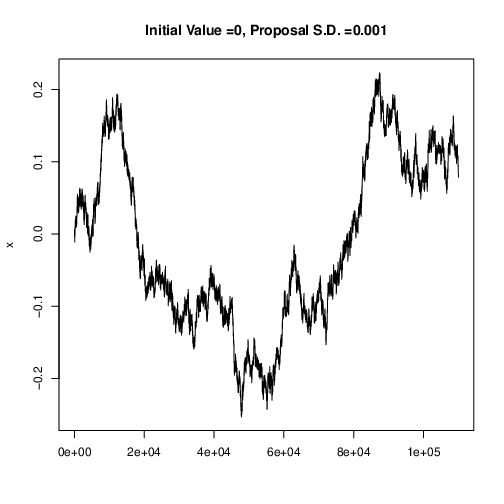
\includegraphics[height=7cm]{./Pics/sp5.png}
\end{center}
\end{frame}
\begin{frame}{Acceptance Rate}
\begin{itemize}
\item The acceptance rate is almost 1.

\item However is this a good proposal?

\item The jumps made by this proposal are too small, and do not sample enough iterates from the tails of the distribution.

\item If it runs long enough the Markov chain will provide a sample from the target distribution.  However, it is very inefficient.
\end{itemize}
\end{frame}
\begin{frame}{Random Walk proposal}
\begin{itemize}
\item For a random walk proposal it is not good to have an acceptance rate that is too high or too low.

\item What exactly is {\em too high} and {\em too low}?

\item It depends on many things including the target and proposal.

\item A rough rule is to aim for an acceptance rate between 20\% and 70\%

\item If your acceptance rate is outside this range the proposal variance can be doubled or halved

\item There are better (but more complicated) ways to do this.
\end{itemize}
\end{frame}
\begin{frame}{Monte Carlo Error}
\begin{itemize}
\item Now that there is a sample. $X^{[1]},X^{[2]},\ldots,X^{[M]}\sim p(x)$. What can it be used for?

\item We can estimate the expected value $E(X)$

\item This can be done by taking:
\begin{equation*}
E(X)\approx \frac{1}{M}\sum_{i=1}^M X^{[i]}
\end{equation*}

\item Note we use $\approx$ instead of $=$.  There is some error since we are estimating $E(X)$ based on a sample.

\item Luckily we can make this smaller by generating a bigger sample.

\item We call this Monte Carlo error.
\end{itemize}
\end{frame}
\begin{frame}{Measuring Monte Carlo Error}
\begin{itemize}
\item One way to measure Monte Carlo Error is the variance of the sample mean.

\begin{align*}
\mbox{Var}\left(\frac{1}{M}\sum_{i=1}^M X^{[i]}\right)&=\frac{1}{M^2} \mbox{Var}\left(\sum_{i=1}^M X^{[i]}\right)\\
&=\frac{1}{M^2} \sum_{i=1}^M\mbox{Var}(X^{[i]})
\only<3>{+\frac{2}{M^2}\sum_{i=1}^M\sum_{j>i}\mbox{cov}(X^{[i]},X^{[j]})}\\
&=\frac{\mbox{Var}(X)}{M}
\only<3>{+\frac{2}{M^2}\sum_{i=1}^M\sum_{j>i}\mbox{cov}(X^{[i]},X^{[j]})}\\
\end{align*}

\item A sample from a Markov chain is {\bf correlated}
\end{itemize}
\end{frame}
\begin{frame}{Monte Carlo efficiency}
\begin{itemize}
\item It is better to have lower correlation in the Markov chain.

\item The efficiency of the chain can be measured using the {\bf effective sample size}.

\item The effective sample size can be computed using the function {\em effectiveSize} in the R Package coda.

\item Obtain an effective sample size for your sample (excluding burn in) where

\begin{itemize}
\item Proposal S.D. =1
\item Proposal S.D. =5
\end{itemize}

\item My answers were about 6000 and 18000 and yours should be close to that
\end{itemize}
\end{frame}
\begin{frame}{Interpret Effective Sample Size}
\begin{itemize}
\item What does it mean to say a Monte Carlo with a sample size of 100000 has an {\bf effective sample size (ESS)} of just 6000?

\item The sampling error of a correlated sample of 100000 is equal to the sampling error of an {\em independent sample} of 6000.

\item Mathematically
\begin{equation*}
\mbox{Var}\left(\frac{1}{M}\sum_{i=1}^M X^{[i]}\right)=\frac{\mbox{Var}(X)}{M}
+\frac{2}{M^2}\sum_{i=1}^M\sum_{j>i}^M\mbox{cov}(X^{[i]},X^{[j]})=\frac{\mbox{Var}(X)}{M_{eff}}
\end{equation*}

\item It is a useful diagnostic for comparing two different proposal variances.  A higher ESS implies a more efficient scheme.
\end{itemize}
\end{frame}
\section{Metropolis-Hastings}
\begin{frame}{Non-Symmetric proposal}
\begin{itemize}
\item In 1970, Hastings proposed an extension to the Metropolis Hastings algorithm.

\item This allows for the case when
\begin{equation}
q(x^{[old]}\rightarrow x^{[new]})\neq q(x^{[new]}\rightarrow x^{[old]})
\end{equation}

\item The only thing that changes is the acceptance probability

\begin{equation}
\alpha=min\left(1,\frac{p(x^{[new]})q(x^{[new]}\rightarrow x^{[old]})}{p(x^{[old]})q(x^{[old]}\rightarrow x^{[new]})}\right)
\end{equation}

\item This is called the {\bf Metropolis-Hastings algorithm }
\end{itemize}
\end{frame}
\begin{frame}{An interesting proposal}
\begin{itemize}
\item Suppose we use the proposal:

\begin{equation}
x^{new}\sim N(0,\sqrt{(5/3)})
\end{equation}

\item What is $q(x^{[old]}\rightarrow x^{[new]})$?

\item It is $q(x^{[new]})$ where $q(.)$ is the density of a  $N(0,\sqrt{(5/3)})$.

\item Is this symmetric?

\item No, since generally $q(x^{[new]})\neq q(x^{[old]})$
\end{itemize}
\end{frame}
\begin{frame}{Metropolis Hastings}
\begin{itemize}
\item Code this where $p(.)$ is the standard t density with 5 d.f, and $q(.)$ is normal with mean 0 and standard deviation 5/3.

\item Inside a loop
\begin{itemize}
  \item Generate $x^{[new]}\sim N(0,\sqrt{(5/3)})$
  \item Set $x^{old}=x^{[i]}$ and compute
  \begin{equation}
  \alpha=min\left(1,\frac{p(x^{[new]})q(x^{[old]})}{p(x^{[old]})q(x^{[new]})}\right)
  \end{equation}
  \item Set $x^{[i+1]}$ to $x^{[new]}$ with probability $\alpha$ (accept)
  \item Set $x^{[i+1]}$ to $x^{[old]}$ with probability $1-\alpha$ (reject)
\end{itemize}

\item Try it
\end{itemize}
\end{frame}
\begin{frame}{Comparison}
\begin{itemize}
\item The Effective Sample Size of this proposal is about 43000 much higher than the best random walk proposal.

\item Why does it work so well?

\item The standard t distribution with 5 df has a mean of 0 and a standard deviation of $\sqrt{(5/3)}$

\item So the $N(0,\sqrt{(5/3)})$ is a good approximation to the standard student t with 5 df.
\end{itemize}
\end{frame}
\begin{frame}{Laplace Approximation}
Using a Taylor expansion of $lnp(x)$ around the point $a$
\begin{equation*}
lnp(x)\approx lnp(a)+\left.\frac{\partial lnp(x)}{\partial x}\right|_{x=a}(x-a)
+\frac{1}{2}\left.\frac{\partial^2 lnp(x)}{\partial x^2}\right|_{x=a}(x-a)^2
\end{equation*}

Let $a$ be the point that maximises $ln p(x)$ and let
\begin{equation}
b=-\left(\left.\frac{\partial^2 lnp(x)}{\partial x^2}\right|_{x=a}\right)^{-1}
\end{equation}
\end{frame}
\begin{frame}
The approximation is
\begin{equation*}
lnp(x)\approx lnp(a)-\frac{1}{2b}(x-a)^2
\end{equation*}

Taking exponential of both sides
\begin{equation*}
p(x)\approx k\times exp\left[-\frac{(x-a)^2}{2b}\right]
\end{equation*}

Any distribution can be approximated by a normal distribution with mean $a$ and variance $b$ where $a$ and $b$ values can be found numerically if needed.
\end{frame}
\begin{frame}{Exercise: Generating from skew normal}
\begin{itemize}
\item The density of the skew normal is

\begin{equation}
p(x)=2\phi(x)\Phi(\delta x)
\end{equation}

where $\phi(x)$ is the density of the standard normal $\Phi(x)$ is the distribution of the standard normal.

\item Using a combination of {\em optim}, {\em dnorm} and {\em pnorm} find the Laplace approximation of the skew normal when $\delta=3$

\item Use it to generate a sample from the skew normal distribution using the Metropolis Hastings algorithm.
\end{itemize}
\end{frame}
\begin{frame}{Indirect method v Metropolis Hastings}
\begin{itemize}
\item Some similarities are:

\begin{itemize}
\item Both require a proposal
\item Both are more efficient when the proposal is a good approximation to the target.
\item Both involve some form of accepting/rejecting
\end{itemize}

\item Some differences are:

\begin{itemize}
\item Indirect method produces an independent sample, MH samples are correlated.
\item Indirect method requires $p(x)/q(x)$ to be finite for all $x$.
\item MH works better when $x$ is a (high-dimensional vector).
\end{itemize}

\item Why?
\end{itemize}
\end{frame}
\section{Multiple variables}
\begin{frame}{Multiple variables}
\begin{itemize}
\item Suppose we now want to sample from a bivariate distribution $p(x,z)$

\item The ideas involved in this section work for more than two variables.

\item It is possible to do a 2-dimensional random walk proposal.  However as the number of variables goes up the acceptance rate becomes lower.

\item Also the Laplace approximation does not work as well in high dimensions.

\item Indirect methods of simulation suffer from the same problem.

\item We need a way to break the problem down.
\end{itemize}
\end{frame}
\begin{frame}{Method of composition}
\begin{itemize}
\item Markov chain methods, allow us to break multivariate distributions down.

\item If it is easy to generate from $p(x)$ then the best way is {\bf Method of composition}.  Generate

\begin{itemize}
\item $x^{[i]}\sim p(x)$
\item $z^{[i]}\sim p(z|x=x^{[i]})$
\end{itemize}

\item Sometimes $p(x)$ is difficult to get
\end{itemize}
\end{frame}
\begin{frame}{Gibbs Sampler}
\begin{itemize}
\item If it is easy to simulate from the conditional distribution $f(x|z)$ then that can be used as a proposal

\item What is the acceptance ratio?

\begin{align*}
\alpha&=\left(1,\frac{p(x^{new},z)p(x^{old}|z)}
{p(x^{old},z)p(x^{new}|z)}\right)\\
&=\left(1,\frac{p(x^{new}|z)p(z)p(x^{old}|z)}
{p(x^{old}|z)p(z)p(x^{new}|z)}\right)\\
&=1
\end{align*}
\end{itemize}
\end{frame}
\begin{frame}{Gibbs Sampler}
\begin{itemize}
\item This gives the Gibbs Sampler

\begin{itemize}
\item Generate $x^{[i+1]}\sim p(x^{[i+1]}|z^{[i]})$
\item Generate $z^{[i+1]}\sim p(z^{[i+1]}|x^{[i+1]})$
\item Repeat
\end{itemize}

\item $x$ and $z$ can be swapped around.

\item It works for more than two variables.

\item Always make sure the conditioning variables are at the current state.
\end{itemize}
\end{frame}
\begin{frame}{Metropolis within Gibbs}
\begin{itemize}
\item Even if the individual conditional distributions are not easy to simulate from, Metropolis Hastings can be used {\em within} each Gibbs step.

\item This works very well because it breaks down a multivariate problem into smaller univariate problems.

\item We will practice some of these algorithms in the context of {\em Bayesian Inference}
\end{itemize}
\end{frame}
\begin{frame}{Summary}
\begin{itemize}
\item You should be familiar with a {\em Markov chain}

\item You should understand this can have a {\em stationary distribution}

\item You should have a basic understanding of the Metropolis Hastings and the special cases

\begin{itemize}
\item Random Walk Metropolis
\item Laplace approximation
\item Gibbs Sampler
\end{itemize}
\end{itemize}
\end{frame}
\end{document}
